\documentclass{article}
\usepackage{graphicx}
\usepackage{hyperref}
\usepackage{changepage}
\usepackage{tikz}
\usepackage{tgtermes}
\usepackage{amsfonts}

\usepackage{fancyhdr}
\pagestyle{fancy}


\usepackage{tikz}
\usepackage{pgfplots}
\usetikzlibrary{positioning}
\usetikzlibrary{arrows}




\renewcommand{\headrulewidth}{0pt}


\fancyhead[L]{DCC 207} 
\fancyhead[R]{Geometrial Computacional} 


\fancyfoot[L]{Trabalho Prático I}
\fancyfoot[R]{Outono de 2025}

\fancyhead[C]{}
\fancyfoot[C]{\thepage}

\begin{document}

\begin{center}
    {
    \Large
    Trabalho Prático I - Geometria Computacional

    DCC 207 - Algoritmos II
    
    }

    Departamento de Ciência da Computação, Instituto de Ciências Exatas, Universidade Federal de Minas Gerais

    Belo Horizonte, Minas Gerais

    Outono de 2025
\end{center}

\begin{flushright}
2022101086  Augusto Guerra de Lima\\
\texttt{augustoguerra@dcc.ufmg.br}\\
2023028234  Cauã Magalhães Pereira\\
\texttt{caua.magalhaes@dcc.ufmg.br}\\
2023028579  Heitor Gonçalves Leite\\
\texttt{heitorleite@dcc.ufmg.br}\\

\end{flushright}
\vspace{1cm}

\begin{adjustwidth}{-1.5cm}{-1.5cm}

\section{Introdução}
\ 

Este trabalho objetiva estudar como estruturas de dados associadas a geometria computacional, a saber, \textit{árvores k-dimensionais}, são empregadas no contexto de georreferenciamento.

Em síntese, foram coletados dados de restaurantes e bares na região de Belo Horizonte. Utilizou-se uma árvore k-dimensional para realizar \textit{buscas ortogonais}, isto é, consultas em subconjuntos retangulares na região da cidade.

A próxima seção tratará de como foi realizada a coleta de dados, como foi implementada a estrutura de dados e como foi criada a interface; A terceira seção discutirá os resultados; As considerações finais e a bibliografia concluirão o texto.

\section{Metodologia}

\subsection{Coleta e processamento de dados}
\ 

Inicialmente, os dados brutos fornecidos pela PBH foram processados para manter apenas os registros associados a bares e restaurantes. Essa filtragem foi realizada a partir de palavras-chave aplicadas à descrição da CNAE principal. Em seguida, os endereços dos estabelecimentos foram convertidos para coordenadas geográficas (latitude e longitude) utilizando a API do \textit{OpenStreetMap} com a biblioteca do \texttt{geopy}, com o auxílio de \textit{RateLimiter} para respeitar os limites de requisição. O processo utilizou cache para evitar reconsultas e paralelização com \textit{ThreadPoolExecutor} para acelerar a geocodificação dos dados.

\subsection{Integração dos dados do Comida di Buteco}
\ 

Foram integradas informações adicionais obtidas manualmente a partir dos dados do festival Comida di Buteco. Para os bares participantes, foram incluídas informações como o nome do prato concorrente, imagem e outras descrições, exibidas dinamicamente no mapa interativo. Essa integração exigiu inferir uma correspondência entre os nomes dos estabelecimentos da base da PBH e os registros do festival.

Isso se deve ao fato de que alguns registros do nome fantasia não coincidirem no \textit{join}, sendo necessário um processo manual de ratificação dos dados.


\subsection{Estrutura de dados, árvore k-dimensional}
\ 

Árvores \(k\)-dimensionais dividem o conjunto \(P\) de pontos em partições. Seja \(p \in P\) um ponto tal que \(p=(x_1,x_2,...,x_k)\), isto é, possui \(k\) coordenadas, a estrutura de dados particiona recursivamente o espaço alternando entre suas dimensões, de forma a comparar apenas uma dimensão específica por nível, resultado em uma \textit{árvore binária}.

Em particular, nos dados geográficos, as coordenadas \textit{latitude} e \textit{longitude} implicam em uma árvore bidimensional (\(2d\)\textit{-tree}); De forma que, se no nível \(l\) é utilizada a coordenada \(x_1\) para o particionamento, em \(l+1\) tão somente, será utilizada a coordenada \(x_2\), tal que \((x_1,x_2) \in \texttt{float}^2\).

A propósito, seja \(a=(a_1,a_2),\ b=(b_1,b_2) \in \texttt{float}^2\), duas coordenadas tal que \(a_1\leq b_1\) e \(a_2 \leq b_2\), o conceito de \textit{busca intervalar ortogonal} surge naturalmente: Constitui-se em determinar um subconjunto de pontos \(P'=\{p_1,p_2,...,p_n\} \subset \texttt{float}^2\), onde 
para todo \(p \in P'\), \(a \leq p \leq b\); Com a adição de que busca é definida em retângulos paralelos aos eixos.

Como mostrado em \cite{md}, a \textit{busca intervalar ortogonal} tem uma propriedade útil, designadamente pode ser decomposta em produto de \textit{buscas intervalares unidimensionais}. Justificando a rotatividade de coordenadas.
\[\{p \in \texttt{float}^k : a_i \leq p_i \leq b_i\} = [a_1,b_1] \times[a_2,b_2] \times ... \times [a_k, b_k].\]

\begin{figure}[h!]
\centering
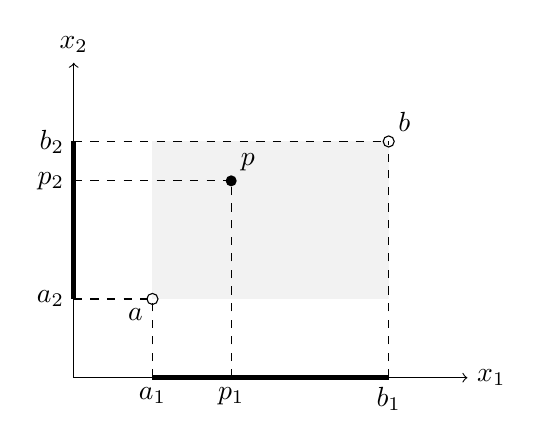
\begin{tikzpicture}

  \draw[->] (0,0) -- (5,0) node[right] {$x_1$};
  \draw[->] (0,0) -- (0,4) node[above] {$x_2$};

  \fill[gray!10] (1,1) rectangle (4,3);
  \draw[line width=2pt] (0,1)--(0,3);
  \draw[line width=2pt] (1,0)--(4,0);
  \draw[dashed] (1,0) -- (1,1);
  \draw[dashed] (4,0) -- (4,3);
  \draw[dashed] (0,1) -- (1,1);
  \draw[dashed] (0,3) -- (4,3);

  % Labels
  \node at (1,0) [below] {$a_1$};
  \node at (4,0) [below] {$b_1$};
  \node at (0,1) [left] {$a_2$};
  \node at (0,3) [left] {$b_2$};
  \node at (1,1) [below left] {$a$};
  \node at (4,3) [above right] {$b$};

  % Point p
  \draw (1,1) circle (2pt);
  \draw (4,3) circle (2pt);
  \fill (2,2.5) circle (2pt);
  \draw[dashed] (2,0) -- (2,2.5);
  \draw[dashed] (0,2.5) -- (2,2.5);
  \node at (2,2.5) [above right] {$p$};
  \node at (2,0) [below] {$p_1$};
  \node at (0,2.5) [left] {$p_2$};
\end{tikzpicture}
\caption{Representação de uma busca intervalar ortogonal em um espaço bidimensional arbitrário.}
\end{figure}

\begin{figure}[h!]
\centering
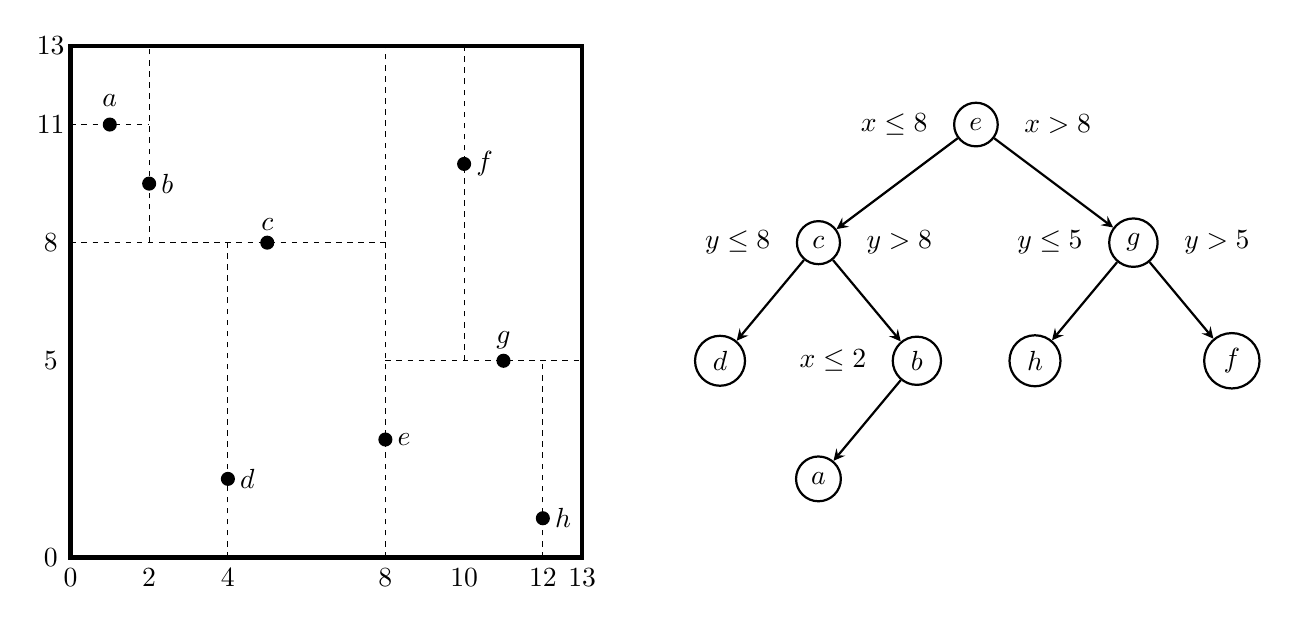
\begin{tikzpicture}[scale=0.5, node distance=0.03cm,
	nosep/.style={inner sep=0pt, outer sep=0pt},
	pt/.style={scale=0.5, circle, minimum size=0.3cm, fill=black, draw=black, thick, nosep},
	line/.style={draw=black, thin, dash pattern=on 2pt},
	grnode/.style={circle, minimum size=0.5cm, fill=white, draw=black, thick},
	arrow/.style={thick, black, -stealth}
]

% Outer rectangle
\draw[ultra thick, black] (0,0)--(13,0)--(13,13)--(0,13)--cycle;

% Selectively label only necessary coordinates
\foreach \x in {0, 2, 4, 8, 10, 12, 13}
	\node at (\x,-0.5) {\x};
\foreach \y in {0, 5, 8, 11, 13}
	\node at (-0.5,\y) {\y};

% Partitioning lines (thin)
\draw[line] (0,11) -- (2,11);
\draw[line] (2,8) -- (2,13);
\draw[line] (0,8) -- (8,8);
\draw[line] (4,0) -- (4,8);
\draw[line] (8,0) -- (8,13);
\draw[line] (8,5) -- (13,5);
\draw[line] (10,5) -- (10,13);
\draw[line] (12,0) -- (12,5);

% Points in black
\node[pt] (a) at (1,11) {};
\node[pt] (b) at (2,9.5) {};
\node[pt] (c) at (5,8) {};
\node[pt] (d) at (4,2) {};
\node[pt] (e) at (8,3) {};
\node[pt] (f) at (10,10) {};
\node[pt] (g) at (11,5) {};
\node[pt] (h) at (12,1) {};

% Point labels
\node[above=of a] (ta) {$a$};
\node[right=of b] (tb) at (2,9.5) {$b$};
\node[above=of c] (tc) at (5,8) {$c$};
\node[right=of d] (td) at (4,2) {$d$};
\node[right=of e] (te) at (8,3) {$e$};
\node[right=of f] (tf) at (10,10) {$f$};
\node[above=of g] (tg) at (11,5) {$g$};
\node[right=of h] (th) at (12,1) {$h$};

% Reset shift for tree (original center)
\tikzset{shift={(23,11)}}

% Tree nodes with white fill, black border
\node[grnode] (ne) at (0,0) {$e$};
\node[grnode] (nc) at (-4,-3) {$c$};
\node[grnode] (ng) at (4,-3) {$g$};
\node[grnode] (nd) at (-6.5,-6) {$d$};
\node[grnode] (nb) at (-1.5,-6) {$b$};
\node[grnode] (nh) at (1.5,-6) {$h$};
\node[grnode] (nf) at (6.5,-6) {$f$};
\node[grnode] (na) at (-4,-9) {$a$};

% Tree edges and decision labels (all black)
\draw[arrow] (ne) -- (nc);
\node[black, left=0.2cm of ne] {$x\leq8$};

\draw[arrow] (ne) -- (ng);
\node[black, right=0.2cm of ne] {$x>8$};

\draw[arrow] (nc) -- (nd);
\node[black, left=0.2cm of nc] {$y\leq8$};

\draw[arrow] (nc) -- (nb);
\node[black, right=0.2cm of nc] {$y>8$};

\draw[arrow] (nb) -- (na);
\node[black, left=0.2cm of nb] {$x\leq2$};

\draw[arrow] (ng) -- (nh);
\node[black, left=0.2cm of ng] {$y\leq5$};

\draw[arrow] (ng) -- (nf);
\node[black, right=0.2cm of ng] {$y>5$};

\end{tikzpicture}
\caption{Visualização de pontos no mapa  e seu particionamento, e a representação da instancia na estrutura de dados utilizada.}
\end{figure}

\subsubsection{Implementação}
\

A estrutura de dados foi implementada em \texttt{C++}. Para integrar com toda a aplicação em \texttt{Python}, foi necessário utilizar o \textit{nanobind}, uma pequena biblioteca de integração dessas duas linguagens de programação.

A árvore k-dimensional foi escrita utilizando índices, ou seja, ela apenas armazena um apontador para onde os dados estão realmente alocados, evitando movimentação em massa dos dados.

A prática de implementar estruturas de dados em \texttt{C++} para realizar a computação de forma mais eficiente e retornar os resultados para a aplicação \texttt{Python} é bastante usual.

% Uso de template

% Como são escolhidos os nos

\subsubsection{Complexidade}
\

Seja \(k\) o número de pontos encontrados em uma \textit{busca intervalar ortogonal}, a complexidade do \textit{tempo de execução} da busca pertence ao conjunto \(\mathcal{O}(\sqrt{n})\), mas reportar todas as ocorrências está em \(\mathcal{O}(\sqrt{n} + k)\).

A cada dois níveis da árvore k-dimensional, o número de nós que podem ser atingidos dobra. A relação de recorrência a seguir modela a discussão; Seja \(T(n)\) o número de nós acessados em uma subárvore com \(n\) pontos.

\(T(n) \leq 2\) se \(n \le 4\); \(T(n) \leq 2T(\frac{n}{4}) + 1\) contrariamente.

Expandindo a recorrência,

\[T(n) \leq 2T(\frac{n}{4}) + 1\]
\[ \ \leq 2(2T(\frac{n}{4^2})+ 1) + 1 \]
\[... \leq \sum_{i=0}^{k-1}2^i + 2^k T(\frac{n}{4^k}) \ \]

\[\Rightarrow T(n) \leq (2^{\log_4 n} -1 ) + 2^{\log_4 n}T(1) \leq 3 \sqrt{n}\]

\[T(n) \in \mathcal{O} (\sqrt{n}).\]


\subsection{Interface interativa e publicação}
\ 

A interface do sistema foi desenvolvida com a biblioteca \textit{dash-leaflet}, que combina os recursos de visualização do \textit{Dash} com a renderização geográfica do \textit{Leaflet}. Foram implementadas funcionalidades de visualização dos estabelecimentos no mapa com pinos georreferenciados, seleção interativa de regiões, atualização da tabela de dados e exibição de detalhes complementares. O sistema final foi publicado em ambiente web utilizando a plataforma \textit{Render}, com o servidor \textit{gunicorn} para servir a aplicação \texttt{Python}.


\section{Resultados}
\ 


\section{Considerações finais}
\ 



\newpage
\section{Bibliografia}

\begin{thebibliography}{99}

\bibitem[CDB]{comida}
Comida di Buteco. Disponível em: \url{https://comidadibuteco.com.br/}. Acesso em: 2 jun. 2025.


\bibitem[DL]{dashleaflet}
\textit{Dash-Leaflet Documentation}. Disponível em: \url{https://dash-leaflet.herokuapp.com/}. Acesso em: 1 jun. 2025.

\bibitem[GB]{guibas}
Leonidas J. Guibas. \textit{Geometric Range Searching
Kinetic Data Structures
Clustering Mobile Nodes}; Stanford University. Disponível em: \url{https://graphics.stanford.edu/courses/cs428-03-spring/03Talks/Range.pdf}. Acesso em: 1 jun. 2025.

\bibitem[GPY]{geopy}
\textit{Geopy Documentation}. Disponível em: \url{https://geopy.readthedocs.io/}. Acesso em: 16 mai. 2025.

\bibitem[MD]{md}
MOUNT, Dave. CMSC 754: \textit{Lecture} 14 \textit{- Orthogonal Range Searching and kd-Trees}; University of Maryland. Disponível em: \url{https://www.cs.umd.edu/class/fall2021/cmsc754/Lects/lect14-kd-tree.pdf}. Acesso em: 1 jun. 2025.

\bibitem[NB]{nb}
\textit{Nanobind Repository}. Disponível em: \url{https://github.com/wjakob/nanobind}. Acesso em: 6 de jun. 2025.

\bibitem[RD]{render}
\textit{Render Documentation}. Disponível em: \url{https://render.com/docs}. Acesso em: 5 jun. 2025.


\end{thebibliography}
\end{adjustwidth}





\end{document}


